
\title{\LaTeX}
\section{\LaTeX}

\begin{frame}[fragile=singleslide]
\label{latex}
\begin{block}{\centering\Large Föreläsning 2 --- \LaTeX}
Förberedelse inför laboration 2.

\begin{itemize}
\item Ordbehandling
\item \LaTeX
\item Mall för rapport
\item Dokumentstruktur: dokumentklasser, omgivningar, text, stycken, listor, tabeller, \ldots
\item Programlistor
\item Matematiska formler
\item Bilder
\end{itemize}
\end{block}
\end{frame} 

\begin{frame}[fragile=singleslide]
\frametitle{Ordbehandling}
De flesta moderna ordbehandlare, till exempel Microsoft Word,  fungerar 
enligt \emph{WYSIWYG}-principen:

\blankline
\begin{center}
What You See Is What You Get
\end{center}

\blankline
Det innebär att det man ser på skärmen ser likadant ut som det som kommer
att skrivas på papperet: teckensnitt, storlekar, avstånd, \ldots

Det innebär också att det inte blir bättre än vad det ser ut
på skärmen (What You See Is \emph{All} You Get).
\end{frame} 

\begin{frame}[fragile=singleslide]
\frametitle{Layout av text}
I de flesta ordbehandlare finns det
formatmallar där man till exempel kan bestämma att alla rubriker på
en viss nivå ska ha ett visst utseende. Om man vill ändra
utseendet på alla rubriker så räcker det att ändra i mallen.

\blankline
Det brukar också finnas möjlighet till automatisk numrering av 
rubriker, automatisk generering av innehållsförteckning och 
sakregister och liknande. 

\blankline
När man skriver matematisk text använder man ofta en ekvationseditor
för att skriva de matematiska symbolerna. Ekvationseditorer är inte
enkla att använda, och slutresultatet brukar inte bli bra.
\end{frame} 

\begin{frame}[fragile=singleslide]
\frametitle{\LaTeX}
Med \LaTeX\ arbetar man på ett helt annat sätt: man skriver 
texten i en vanlig textfil och lägger
in \emph{kommandon} (''taggar'')  i texten som visar hur texten ska
formateras. Textfilen kan bli något svårläst, åtminstone innan man är van, men resultatet blir garanterat snyggt.

\blankline
Enkelt exempel:

\begin{exempel}
Pythagoras sats ser ut så
här: $a^2 + b^2 = c^2$.
\end{exempel} 

\code{\$}-tecknen anger att en matematisk formel börjar och slutar. 
\LaTeX\ vet då att variablerna a, b och c ska skrivas kursiva, hur stora
exponenterna ska vara och var de ska placeras, och hur
mycket mellanrum det ska vara mellan termerna.

\end{frame} 

\begin{frame}[fragile=singleslide]
\frametitle{Ett större exempel}
\begin{mexempel}
   If $f$ is continuous on the
   closed interval $a \leq x \leq b$
   and differentiable on the open
   interval $a < x < b$, then there
   exists a point
   $\xi$, $a < \xi < b$ such that
   \begin{displaymath}
      f(b) - f(a) = f'(\xi)(b -a).
   \end{displaymath}
\end{mexempel}

\end{frame} 

\begin{frame}[fragile=singleslide]
\frametitle{\LaTeX-historik}
Donald E. Knuth skrev 1977--1982 typsättningsprogrammet \TeX
\footnote{\TeX\ skrivs TeX i skrivmaskinsskrift och uttalas
''tech''.} 
eftersom han inte var nöjd med de möjligheter till typsättning
som fanns då.

\TeX\ är ett ''lågnivåspråk''. Leslie Lamport byggde på \TeX\ 
med ett makropaket som gör det möjligt för författaren av ett
dokument att koncentrera sig på den logiska strukturen hos
dokumentet och på själva texten i stället för på lågnivåtypsättningen. 
Resultatet
blev \LaTeX
\footnote{\LaTeX\ skrivs LaTeX i skrivmaskinsskrift och uttalas
''lah-tekh'' eller "lay-tekh".}.

En föregångare till \LaTeX, \emph{troff}, används fortfarande
ibland, till exempel till Unix man-sidor.
\end{frame} 

\begin{frame}[fragile=singleslide]
\frametitle{Arbeta med \LaTeX}
När man använder \LaTeX\ utgår man från en fil med text och kommandon. Filen ska ha tillägget \code{.tex}, till exempel \code{rapport.tex}. Sedan ''översätter'' man filen till \code{pdf}-format med programmet \code{pdflatex} och tittar på resultatet med en pdf-läsare, till exempel \code{evince}. Detta kan man naturligtvis göra genom att skriva kommandona för hand (\code{gedit rapport.tex}, \code{pdflatex rapport.tex}, \code{evince rapport.pdf}), men det är enklare att använda ett specialprogram. På studentdatorerna finns programmet \code{texmaker}. På Mac-datorer använder man t.ex. TeXShop eller TeXstudio som även finns för Windows.

\pindent I stället för att generera pdf-filer med \code{pdflatex} kan man generera dvi-filer (''device independent'') med programmet \code{latex} som man kan titta på med en ''dvi-läsare'' och sedan översätta till Postscript eller pdf. Numera använder de flesta \code{pdflatex}.
\end{frame} 

\begin{frame}[fragile=singleslide]
\frametitle{Mall för rapport}
\vspace{-2mm}
\bex 
\documentclass[a4paper]{article}
\usepackage[T1]{fontenc}
\usepackage[utf8]{inputenc}
\usepackage[swedish]{babel}
\usepackage{fancyvrb}
\fvset{tabsize=4}
\fvset{fontsize=\small}
\title{Programmeringsteknik\\
   Inlämningsuppgift 1}
\author{Xerxes Yngvesson\\
   dat14xyn@student.lu.se}
\date{2014--10--17}

\begin{document}
\maketitle

Här skriver man texten i
rapporten.
\end{document}
\end{verbatim}
\mex
\begin{center}
\LARGE Programmeringsteknik \\
\LARGE \ Inlämningsuppgift 1\\
\blankline
\large Xerxes Yngvesson \\
\large dat14xyn@student.lu.se\\
\large 2014--10--17
\end{center}
\vspace{1cm}
Här skriver man texten i
rapporten.
\eex
\end{frame} 

\begin{frame}[fragile=singleslide]
\frametitle{Dokumentklasser och omgivningar}
\verb+{article}+ är en \emph{dokumentklass} (den man oftast använder). 
Andra dokumentklasser är \verb+{report}+,
\verb+{book}+, \verb+{letter}+ och \verb+{beamer}+ (beamer används för overheadbilder). En dokumentklass
påverkar utseendet på hela dokumentet.

\blankline
\verb+\begin{document}+ definierar starten på en \emph{omgivning},
\verb+\end{document}+ slutet på omgivningen. En omgivning påverkar
utseendet på den del av dokumentet som ingår i omgivningen.
Vi kommer att se exempel på andra omgivningar senare. 
\end{frame} 

\begin{frame}[fragile=singleslide]
\frametitle{Löpande text}
Radslut och antal mellanslag mellan ord har ingen betydelse,
\LaTeX\ formaterar så att det blir snyggt. En
eller flera blanka rader ger ett nytt stycke. Exempel:

\bex
Det här
är en text som jag
har    skrivit. Det är
en lång text med flera
rader.

Här börjar det ett
nytt stycke i texten.
\end{verbatim}
\mex
Det här
är en text som jag
har    skrivit. Det är
en lång text med flera
rader.

\hspace{1em}Här börjar det ett
nytt stycke i texten.
\eex
\end{frame} 

\begin{frame}[fragile=singleslide]
\frametitle{Rubriker}
\LaTeX\ numrerar rubriker automatiskt. Man anger en rubrik med
\verb+\section+ eller \verb+\subsection+.

\bex 
\section{Inledning}
\section{Utförande}
\subsection{Del 1}
\subsection{Del 2}
\section{Slutsatser}
\end{verbatim}
\mex
{\Large\bfseries 1 Inledning} \\[1ex]
{\Large\bfseries 2 Utförande} \\[1ex]
{\large\bfseries 2.1 Del 1} \\[1ex]
{\large\bfseries 2.2 Del 2} \\[1ex]
{\Large\bfseries 3 Slutsatser}
\eex

\end{frame} 

\begin{frame}[fragile=singleslide]
\frametitle{Ändra textens utseende}
Det finns många kommandon för att ändra utseende på texten. Två 
sådana kommandon  är \verb+\emph+ för att betona text och \verb+\texttt+
för att skriva med skrivmaskinstypsnitt. Exempel:

\begin{exempel}
Här skriver jag något
\emph{viktigt}. Och 
i Java har vi använt
klassen \texttt{Square}.
\end{exempel}

Det finns också kommandon för fetstil, lutande text, osv, och för att
ändra storlek på texten. Använd sparsamt!
\end{frame} 

\begin{frame}[fragile=singleslide]
\frametitle{Specialtecken}
Med tecknet \code{\%} inleder man en kommentar som sträcker sig till slutet av raden.

\blankline
En del tecken används för kommandon och måste skrivas på speciellt sätt:

\begin{Code}
\$ \% \_ \# \& \{ \} \textbackslash
\end{Code}

Det finns streck, mellanrum och punkter av olika slag:

\begin{exempel}
DoD-kursen pågår under vecka
1--3 av läsperiod ht1. Tyvärr 
är den inte längre \ldots

\quad Telefon: 046--222~80~38.
Dagens datum: \today.
\end{exempel}
\end{frame} 

\begin{frame}[fragile=singleslide]
\frametitle{Fotnoter}
Fotnoter är lätta att skriva:

\bex 
Om man använder \LaTeX
\footnote{uttalas 
''lah-tekh''} så
blir det bra. Alla rapporter
blir automatiskt snyggt
utformade.
\end{verbatim}
\mex
Om man använder \LaTeX
\footnote{uttalas 
''lah-tekh''} så
blir det bra. Alla rapporter
blir automatiskt snyggt
utformade.
\eex

Fotnoter numreras automatiskt 1,2,\ldots 
Fast här blev ''numret'' på fotnoten ''a'' av olika anledningar.
Observera att man skriver två apostrofer (\verb+''+) i stället
för citationstecken (\code{"}).
\end{frame} 

\begin{frame}[fragile=singleslide]
\frametitle{Listor}
Punktlistor är enkla:

\begin{exempel}
\begin{itemize}
  \item första punkten
  \item här kommer den andra 
  punkten i listan
\end{itemize}
\end{exempel}

Numrerade listor är lika enkla:

\begin{exempel}
\begin{enumerate}
  \item första punkten
  \item här kommer den andra
  punkten i listan
\end{enumerate}
\end{exempel}

OBS! Pga hur detta dokument är formaterat så får listelementen inga punkter eller siffror, men i den vanliga dokumentklassen \code{\{article\}} blir det som förväntat.
% I detta dokument används dokumentklassen \code{beamer}, och där blir numren siffror i cirklar. I den vanliga dokumentklassen \code{\{article\}} blir numren 1., 2., \ldots
\end{frame} 

\begin{frame}[fragile=singleslide]
\frametitle{Definitioner}
\begin{exempel}
Några klasser som vi använder:

\begin{description}
\item[SimpleWindow] Beskriver ett
enkelt ritfönster
\item[Scanner] Inläsning från 
tangentbordet
\item[Random] Slumptal
\end{description}
\end{exempel}

I dokumentklassen \code{article} blir det något annorlunda layout på definitioner. Använd en \code{tabular}-omgivning med kolumnspecifikationen \code{p\{bredd\}} för att få layout som liknar den ovan.
\end{frame} 

\begin{frame}[fragile=singleslide]
\frametitle{Tabeller}
En tabell där den första kolumnen är vänsterinpassad (\code{l}), den 
andra centrerad (\code{c}) och den tredje högerinpassad (\code{r}). \code{\&} avgränsar kolumnerna, 
\verb+\\+ betyder ny rad, \verb+~+ är ett ''hårt'' blanktecken. \verb+\hline+ är ett streck.

\bex
\begin{tabular}{lcr}
  Produkt  & Typ    & Pris    \\
  \hline
  Skruvar  & stora  & 0.18~kr \\
  Muttrar  & M16    & 0.38~kr \\
  Spikar   & 12~tum & 0.12~kr
\end{tabular}
\end{verbatim}
\mex
\begin{tabular}[t]{lcr}
  Produkt  & Typ    & Pris    \\
  \hline
  Skruvar  & stora  & 0.18~kr \\
  Muttrar  & M16    & 0.38~kr \\
  Spikar   & 12~tum & 0.12~kr
\end{tabular}
\eex
\end{frame} 

\begin{frame}[fragile=singleslide]
\frametitle{Flytande tabeller}
Med en \verb+\table+-omgivning skapar man en tabell med en förklarande
text och ett nummer. \LaTeX\ placerar tabellen där det är 
lämpligt.

\bex
\begin{table}
\begin{tabular}{lcr}
  Produkt  & Typ    & Pris    \\
  \hline
  Skruvar  & stora  & 0.18~kr \\
  Muttrar  & M16    & 0.38~kr \\
  Spikar   & 12~tum & 0.12~kr
\end{tabular}
\caption{Våra produkter}
\end{table}
\end{verbatim}
\mex
\begin{tabular}[t]{lcr}
  Produkt  & Typ    & Pris    \\
  \hline
  Skruvar  & stora  & 0.18~kr \\
  Muttrar  & M16    & 0.38~kr \\
  Spikar   & 12~tum & 0.12~kr
\end{tabular}
\begin{center}
{Tabell 7. Våra produkter}
\end{center}
\eex
\end{frame} 

\begin{frame}[fragile=singleslide]
\frametitle{Att referera till etiketter}
Om man sätter en etikett på en tabell kan man referera till den
från texten. Exempel: 

\bex
\begin{table}
\begin{tabular}{lcr}
  Produkt  & Typ    & Pris    \\
  \hline
  Skruvar  & stora  & 0.18~kr \\
\end{tabular}
\caption{Våra produkter}
\label{produkter}
\end{table}
Senare i texten: våra produkter
finns i tabell~\ref{produkter}.
\end{verbatim}
\mex
\begin{tabular}[t]{lcr}
  Produkt  & Typ    & Pris    \\
  \hline
  Skruvar  & stora  & 0.18 kr \\
\end{tabular}
\begin{center}
{Tabell 7. Våra produkter}
\end{center}
Senare i texten: våra produkter
finns i tabell~7.
\eex
Figurer hanteras likadant som tabeller, i en 
\verb+\figure+-omgivning.
\end{frame} 

\begin{frame}[fragile=singleslide]
\frametitle{Programlistor}
För att infoga en programlista i en rapport använder man
kommandot \verb+\VerbatimInput{filnamn}+ från paketet
\texttt{fancyvrb}. Man bör \emph{inte} använda ''standard''-
kommandot \verb+\verbatiminput+ eftersom det kommandot
ignorerar alla tabulatortecken i programmet, och det medför att
indragningarna försvinner.

\bex
\usepackage{fancyvrb}
\fvset{tabsize=4}
\fvset{fontsize=\small}

\VerbatimInput{Point.java}
\end{verbatim}
\mex
%\vspace{-30pt}
\begin{verbatim}
class Point {
    private int x;
    private int y;

    public Point(int x, int y) {
        this.x = x;
        this.y = y;
    }
}
\end{verbatim}
\eex
\end{frame} 

\begin{frame}[fragile=singleslide]
\frametitle{Öka eller minska avstånd}
Ibland behöver man öka avståndet i vertikalled mellan två avsnitt i texten, till exempel före eller efter en tabell. Det kan man göra med kommandot \verb/\vspace{längd}/, där längden kan anges i millimeter eller punkter eller något annat som \LaTeX\ känner igen. Längden kan vara negativ om man vill minska avståndet. Det finns också specialkommandon för att lägga in ett litet, mellanstort och stort avstånd:

\begin{Code}
\smallskip  \medskip  \bigskip
\end{Code}

Man kan öka eller minska horisontellt avstånd med \verb/\hspace{längd}/.
\end{frame} 

\begin{frame}[fragile=singleslide]
\frametitle{Matematiska formler}
\LaTeX\ är \emph{mycket} bra på att formatera matematisk text. 
Alla (tror jag) artiklar och böcker som innehåller matematiska formler 
är skrivna med \LaTeX. Man kan skriva
formler antingen inuti löpande text eller på en egen rad:
\begin{itemize}
\item I texten: formeln inleds med \code{\$} och avslutas med \code{\$}.
\item På egen rad: formeln inleds med \verb+\begin{displaymath}+
och avslutas med \verb+\end{displaymath}+.
\verb+\begin{equation}+ och \verb+\end{equation}+ ger samma
resultat men formeln numreras. Med \verb+\label+ och \verb+\ref+
kan man etikettera och referera till ekvationer.
\end{itemize}
\end{frame} 

\begin{frame}[fragile=singleslide]
\frametitle{Enkla formler}
\begin{mexempel}
Formeln $x=3y-2$ står 
inne i texten. Däremot
står
\begin{displaymath}
  x=3y-2
\end{displaymath}
för sig själv precis som
\begin{equation}
  x=3y-2
  \label{xochy}
\end{equation}
I ekvation~\ref{xochy} fann
vi att \ldots
\end{mexempel}
\end{frame} 

\begin{frame}[fragile=singleslide]
\frametitle{Symboler, index}
\begin{mexempel}
\begin{displaymath}
\alpha \leq \pi \approx 3.141592654
\end{displaymath}
\end{mexempel}

\vspace{1cm}

\begin{mexempel}
\begin{displaymath}
x_{k+1}=x_{k}-f(x_{k})/f'(x_{k})
\end{displaymath}
\end{mexempel}
\end{frame} 

\begin{frame}[fragile=singleslide]
\frametitle{Exponenter, rötter}
\begin{mexempel}
\begin{displaymath}
e^x = 1+x+x^2/2!+x^3/3!+\cdots
\end{displaymath}
\end{mexempel}

\vspace{1cm}

\begin{mexempel}
\begin{displaymath}
x_{1,2}=\frac{p}{2}\pm
\sqrt{\frac{p^2}{4}-q}
\end{displaymath}
\end{mexempel}

\end{frame} 



\begin{frame}[fragile=singleslide]
\frametitle{Integraler, summor}
\begin{mexempel}
\begin{displaymath}
\int_{-\infty}^{\infty}
e^{-x^2} dx
\end{displaymath}
\end{mexempel}

\vspace{1cm}

\begin{mexempel}
\begin{displaymath}
\sum_{k=1}^n\frac{1}{a_k}
\end{displaymath}
\end{mexempel}

\end{frame} 

\begin{frame}[fragile=singleslide]
\frametitle{Funktioner}
\begin{mexempel}
\begin{displaymath}
  \sin^2 x + \cos^2 x = 1
\end{displaymath}
\end{mexempel}
\end{frame} 

\begin{frame}[fragile=singleslide]
\frametitle{Matriser, parenteser}
\begin{mexempel}
\begin{displaymath}
A=\left(
\begin{array}{cccc}
a_{11} & a_{12} & \cdots & a_{1n}\\
a_{21} & a_{22} & \cdots & a_{2n}\\
\vdots & \vdots & \ddots & \vdots\\
a_{n1} & a_{n2} & \cdots & a_{nn}\\
\end{array}
\right)
\end{displaymath}
\end{mexempel}
\end{frame} 

\begin{frame}[fragile=singleslide]
\frametitle{Bilder}
Bilder kan inkluderas i \LaTeX-dokument om de är i formatet
\code{pdf}, \code{jpeg} eller \code{png} (\texttt{eps} om man använder \code{latex}). Man måste använda paketet \texttt{graphicx} (eller \code{graphics}).
\vspace{20mm}
\bex
\usepackage{graphicx}


\includegraphics[height=40mm]{images/bild.pdf}
\end{verbatim}
\mex
  \vspace{-25mm}\hspace{15mm}
  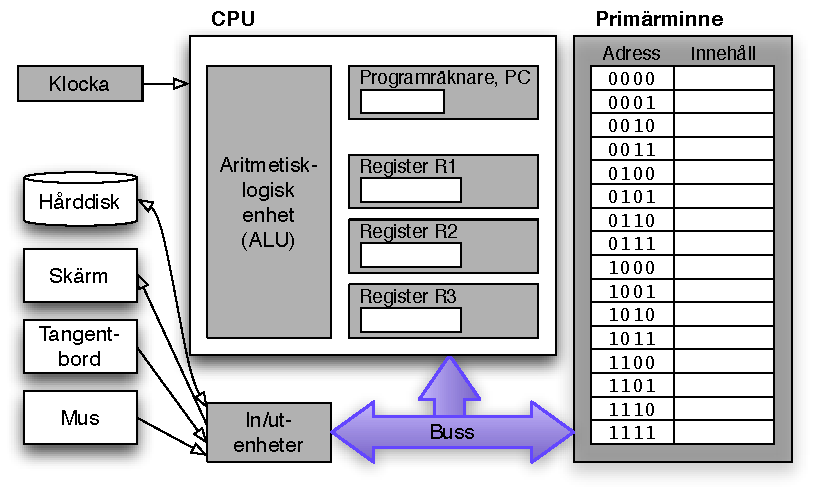
\includegraphics[height=30mm]{images/enkelmodell.pdf}
\eex

ImageMagick-programmet \texttt{convert} kan konvertera
från och till de flesta bildformat:
\begin{verbatim}
   convert bild.fig bild.pdf
\end{verbatim}
\end{frame} 

\begin{frame}[fragile=singleslide]
\frametitle{Egna kommandon}
Man kan lätt definiera egna kommandon, till exempel ett kortare namn
för en text som man använder ofta. Kommandon kan ha parametrar.

\vspace{10mm}

\begin{mexempel}
\newcommand{\java}[1]
{\texttt{#1}}

Klasser: \java{Random}, 
\java{Scanner} och 
\java{PrintStream}.
\end{mexempel}

\vspace{10mm}

Man kan definiera om existerande kommandon med
\verb+\renewcommand+. Det kan ställa till förvirring, så
gör inte det.
\end{frame} 

%\begin{frame}[fragile=singleslide]
%\frametitle{\LaTeX\ på egen dator}
%
%En sammanfattning av LaTeX-installationer finns på \url{www.latex-project.org}, sidan Getting LaTeX.
%
%\begin{description}
%\item[Linux] LaTeX kanske redan finns på datorn; hämtas annars med den vanliga pakethanteraren.
%\item[Mac] Använd MacTeX (bygger på TeXLive, som uppdateras varje år).
%\item[Windows] proTeXt verkar vara enklast.
%\end{description}
%
%Som IDE rekommenderas Texmaker (\url{www.xm1math.net/texmaker}) eller TeXShop (bara för Mac, \url{www.texshop.org}).
%\end{frame} 

